\Needspace{18\baselineskip}

\vfill
\begin{minipage}{\textwidth}

\parttitlewithbox{\textbf{\LARGE Crédits}}

\vspace{2em}

\large{\textbf{Auteur(s):}\\}
\makeatletter
{\robotoCondensed \small{\@author}}
\makeatother

\noindent\textcolor{secondarycolor}{\rule{\linewidth}{0.5pt}}
\vspace{-1em}

\begin{tikzpicture}
    \node[inner sep=0em, text width=\textwidth, align=left] (box) at (0,0) {
\noindent
\begin{minipage}[c]{2cm}
  \centering
  
\includegraphics[width=2cm]{img/CNED-Banniere.png}
\end{minipage}\hfill
\begin{minipage}[c]{14cm}
  \begin{spacing}{0.2}
  {\robotolite\fontsize{6}{1}\selectfont
  Les cours du Cned sont strictement réservés à l’usage privé de leurs destinataires et ne sont pas destinés à une utilisation collective.
  Les personnes qui s’en serviraient pour d’autres usages, qui en feraient une reproduction intégrale ou partielle, une traduction sans
  le consentement du Cned, s’exposeraient à des poursuites judiciaires et aux sanctions pénales prévues par le Code de la propriété
  intellectuelle. Les reproductions par reprographie de livres et de périodiques protégés contenues dans cet ouvrage sont effectuées
  par le Cned avec l’autorisation du Centre français d’exploitation du droit de copie (20, rue des Grands-Augustins, 75006 Paris).}
  \end{spacing}
\end{minipage}\hfill
\begin{minipage}[c]{0.8cm}
  \centering
  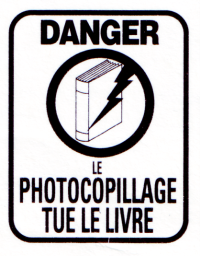
\includegraphics[width=1cm]{img/photocopillage.png}
\end{minipage}

\begin{minipage}[c]{15cm}
  \begin{spacing}{0.5}
  {\robotoMedium\fontsize{6}{9}\selectfont {Cned, BP 60200, 86980 Futuroscope Chasseneuil Cedex, France}
  
\vspace{0.4em}

  \robotolite{Le Cned remercie les personnes qui ont contribué à la réalisation de ce document. Qu’elles trouvent ici l’expression de toute sa reconnaissance}\\

  \vspace{1em}

  © Cned \the\year \hspace{2em} \textit{Ce document peut présenter des défauts d'accessibilité.}
  \hfill
  \codeArticle\\
  }
  \end{spacing}
\end{minipage}
    };
\end{tikzpicture}

\vspace{-1.5em}

\end{minipage}